\RequirePackage[l2tabu, orthodox]{nag}
\documentclass{article}

\usepackage[letterpaper, margin=1.3cm]{geometry}
\usepackage{booktabs}
\usepackage[final]{pdfpages}

\title{ECE 487 Assignment 1}
\author{Michael Kwok}
\begin{document}

\maketitle
\subsection*{Links requied to connect 15 nodes}
\begin{itemize}
    \item Mesh: \((15 * 14) / 2 = 105\)
    \item Star: 15
    \item Bus: 15
    \item Ring: 15
\end{itemize}

\subsection*{Topology diagram}

Attached on 2nd page.

\subsection*{Match to layer}
\begin{itemize}
    \item Transport
    \item Data Link
    \item Transport
    \item Presentation
\end{itemize}

\subsection*{Data frame headers}
\begin{tabular}{ l  c  c  c  c }
    \toprule
                   & \multicolumn{2}{c}{Data frame from PC2 to the router} & \multicolumn{2}{c}{Data frame from router to PC3}                                        \\
    \midrule
                   & Source address                                        & Destination address                               & Source address & Destination address \\
    \midrule
    Layer 2 Header & 25                                                    & 67                                                & 38             & 46                  \\
    Layer 3 Header & C                                                     & B                                                 & B              & B                   \\
    Layer 4 Header & k                                                     & m                                                 & k              & m                   \\
    \bottomrule
\end{tabular}
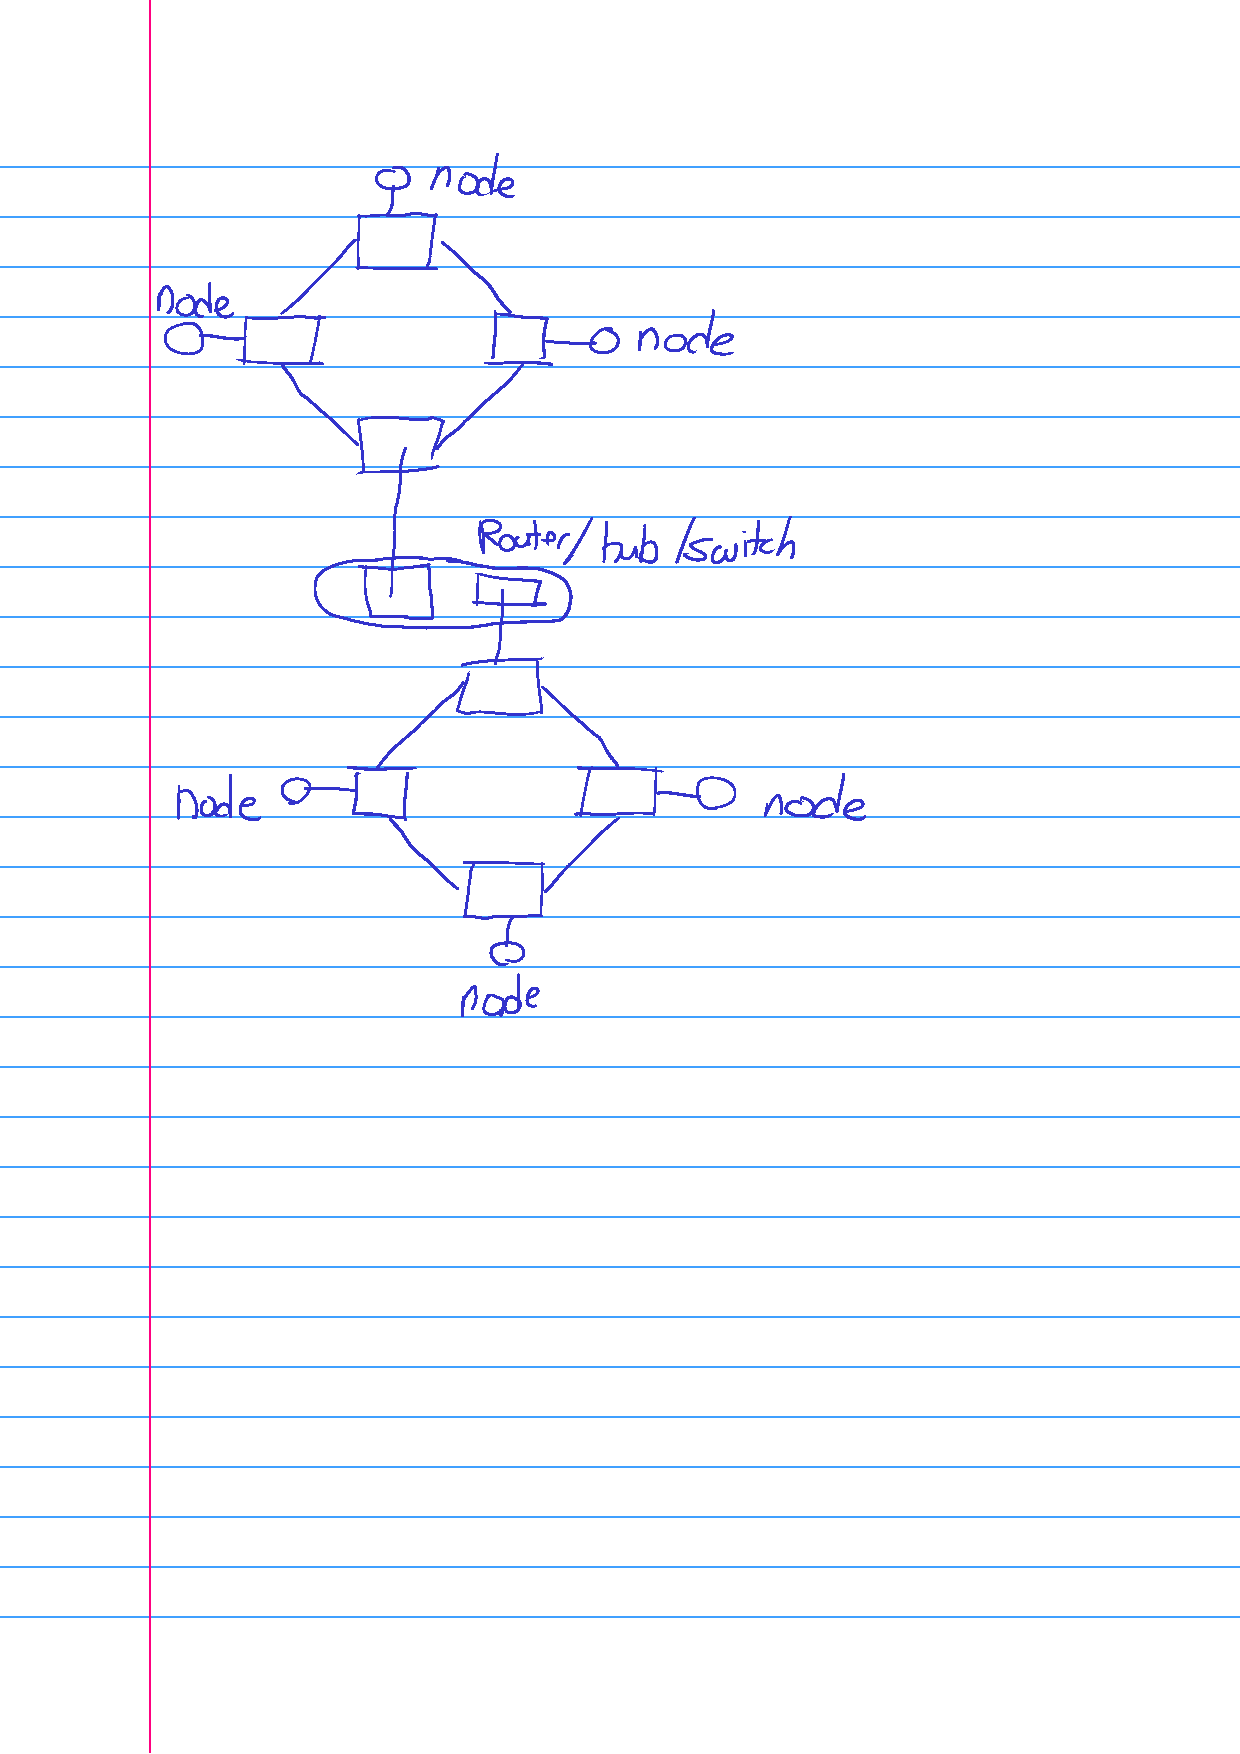
\includepdf[pages=-]{StarRing.pdf}
\end{document}
